\newpage
\section{Auswertung}
\label{sec:Auswertung}
\subsection{Statische Messung}
\begin{figure}[h!]
	\label{fig:overview1}
	\centering
	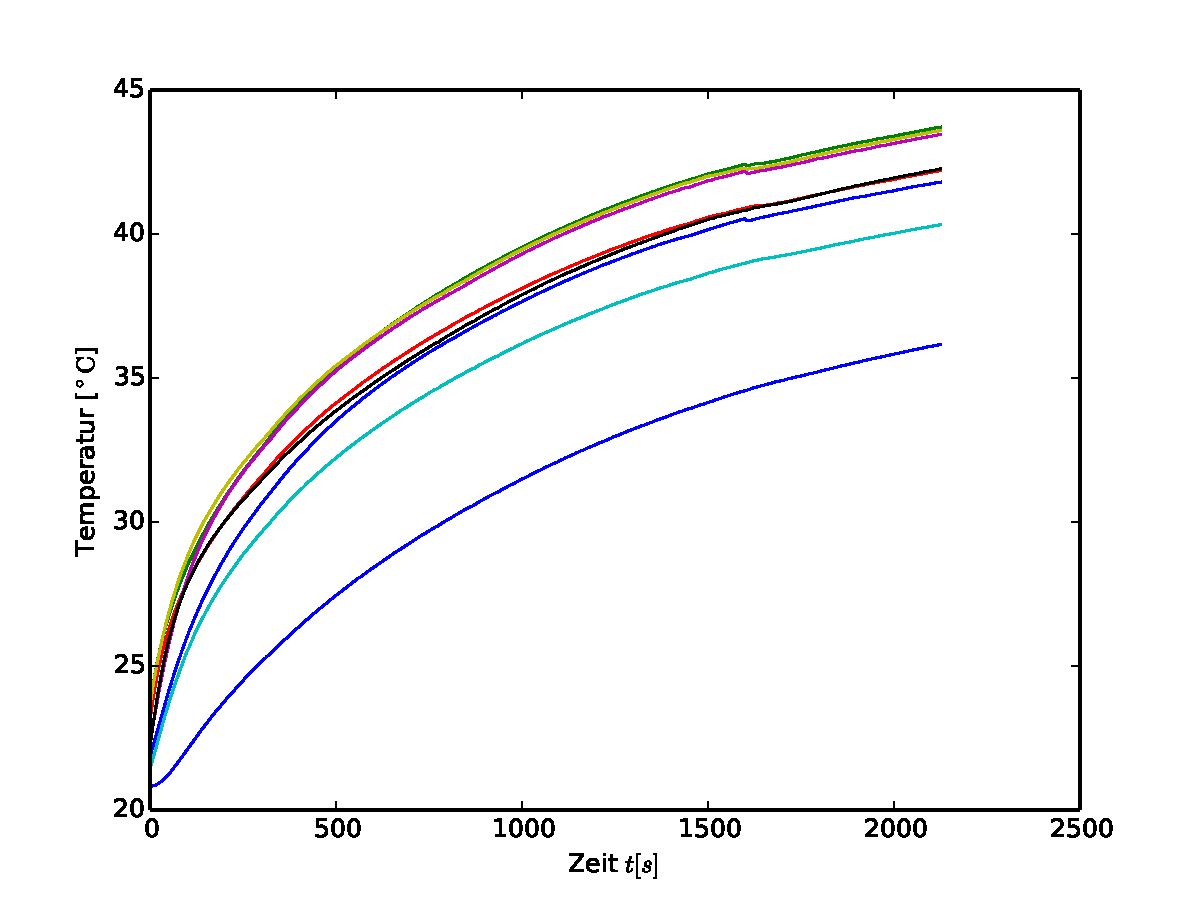
\includegraphics[width=0.8\textwidth]{Bilder/M1_Overview.pdf}
	\caption{Alle gemessenen Temperaturen}
\end{figure}
Alle Temperaturverläufe werden in Diagramm \ref{fig:overview1} gleichzeitig aufgetragen. Es zeigt, dass der allgmeine Verlauf der Temperatur unabhängig von dem Material und der Entfernung des Messpunktes ist. Die Temperaturkurven zeigen jeweils beschränktes Wachstum.

\begin{figure}[p]
	\label{fig:entftemp}
	\centering
	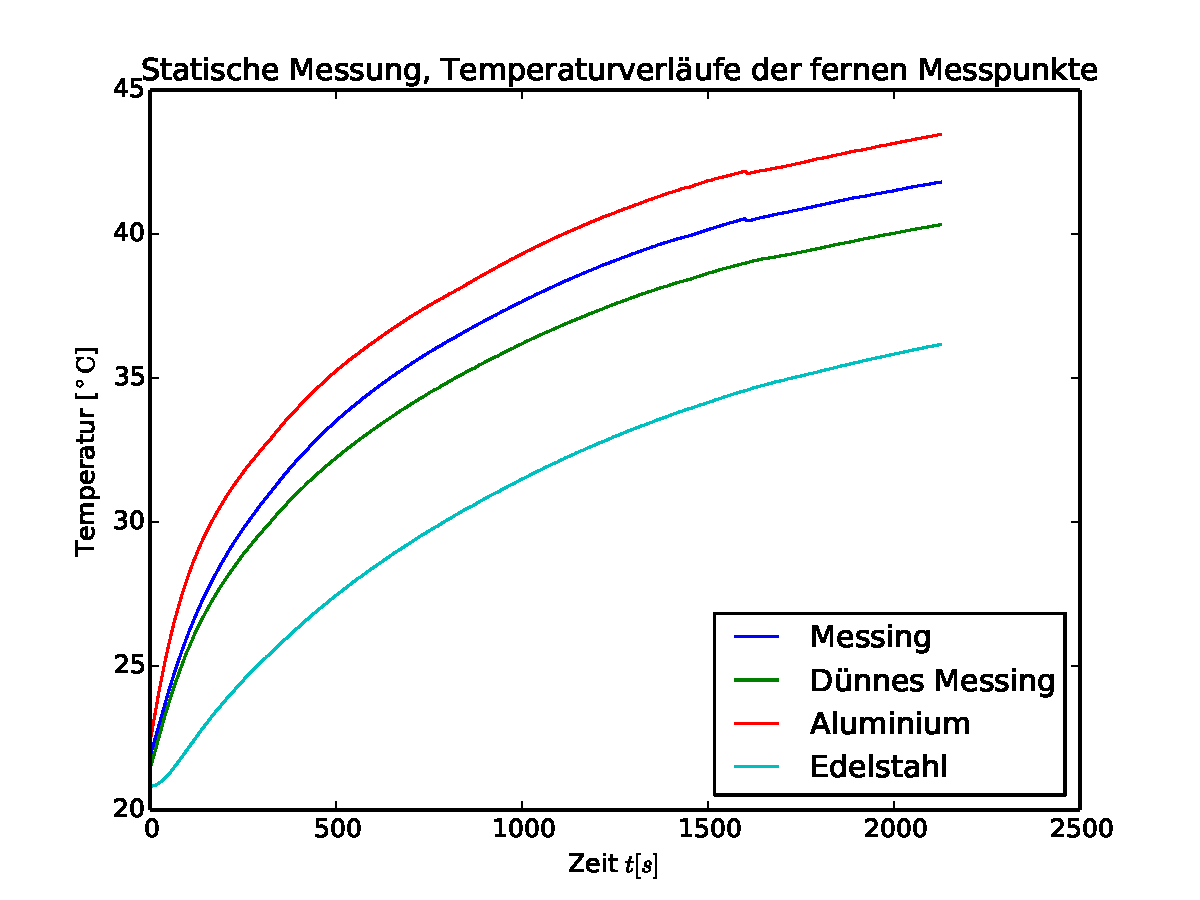
\includegraphics[width=0.8\textwidth]{Bilder/M1_Tempverl.pdf}
	\caption{Verlauf der Temperaturen an den entfernten Messpunkten}
\end{figure}
Im Diagramm \ref{fig:entftemp} wird der Temperaturverlauf bei den entfernten Messpunkte T1, T4, T5, T8 (vgl. \ref{fig:platine}) gezeigt. 
Die Kurve von Aluminium hat zu Beginn des Experiments den stärksten Anstieg und liegt über die der anderen Metallstäbe. 
Beide Kurven der Messingstäbe haben vergleichbare Steigungen;
die Kurve des größeren Messingstabes liegt dabei über der des kleineren Stabes und hat am Endpunkt der Messung zu dieser eine Temperaturdifferenz von etwa $1 \si{\degreeCelsius}$. 
Die Kurve von Edelstahl ist deutlich von den Kurven der anderen Metallstäbe entfernt und weist die geringste Steigung auf. 
Zum Endpunkt der Messung liegt zwischen den Messpunkten von Aluminium und Edelstahl eine maximale Temperaturdifferenz von etwa $7 \si{\degreeCelsius}$ vor. 

Zirka 700 Sekunden nach Beginn des Erwärmens liegen an den entfernten Messpunkten die Temperaturen nach Tabelle \ref{tab:700} vor. 
\begin{table}
\centering
\begin{tabular}{cccc}
	\toprule
	{Edelstahl}&{Messing,dünn}&{Messing}&{Aluminium}\\
	\midrule
	29$\si{\degreeCelsius}$& 34$\si{\degreeCelsius}$& 35.4$\si{\degreeCelsius}$& 37$\si{\degreeCelsius}$\\
	\bottomrule
\end{tabular}
\label{tab:700}
\caption{Temperaturen an entfernten Messpunkten bei $t=700\si{\second}$}
\end{table}
Die höchste Temperatur hat der Aluminiumstab, die geringste Temperatur hat der Edelstahlstab.

Mit 
\begin{equation}
	\mathup{d}Q = -\kappa A\frac{\partial T}{\partial x}\mathup{d}t
	\label{eq:skr1}
\end{equation}
kann der Wärmestrom $\frac{\Delta{Q}}{\Delta{t}}$ innerhalb der Stäbe bestimmt werden. 
Hierzu sind $\kappa$ in \ref{eq:skr1} die Literaturwerte der Wärmeleitfähigkeit und $A$ die Querschnittsfläche (vgl. hierzu \cite{V204}) des jeweiligen Stabes; $\frac{\partial T}{\partial x}$ ist der Temperaturgradient innerhalb des Stabes und wird hier mit $\frac{\Delta T}{\Delta x}$ und $\Delta x=$genähert.
Es ergibt sich\\
\begin{table}
\centering
\begin{tabular}{ccccc}
	\multicolumn{5}{c}{Messing}\\
	\toprule
	Nach $500\si{\second}$&Nach $1000\si{\second}$& Nach $1500\si{\second}$&Nach $2000\si{\second}$& Nach $50\si{\second}$\\
	$-0.3552\si{\watt}$&$-0.36288\si{\watt}$&$-0.37248\si{\watt}$&$-0.3648\si{\watt}$&$-0.49728\si{\watt}$\\
	\bottomrule
\end{tabular}
\end{table}
\begin{table}[h!]
\centering
\begin{tabular}{ccccc}
	\multicolumn{5}{c}{Messing, dünn}\\
	\toprule
	Nach $500\si{\second}$&Nach $1000\si{\second}$& Nach $1500\si{\second}$&Nach $2000\si{\second}$& Nach $50\si{\second}$\\
	$-0.2128\si{\watt}$&$-0.21504\si{\watt}$&$-0.21728\si{\watt}$&$-0.21056\si{\watt}$&$-0.28672\si{\watt}$\\
	\bottomrule
\end{tabular}
\end{table}
\begin{table}[h!]
\centering
\begin{tabular}{ccccc}
	\multicolumn{5}{c}{Aluminium}\\
	\toprule
	Nach $500\si{\second}$&Nach $1000\si{\second}$& Nach $1500\si{\second}$&Nach $2000\si{\second}$& Nach $50\si{\second}$\\

	$-0.06768\si{\watt}$&$-0.0564\si{\watt}$&$-0.0564\si{\watt}$&$-0.04888\si{\watt}$&$-0.41736\si{\watt}$\\
	\bottomrule
\end{tabular}
\end{table}
\begin{table}[h!]
\centering
\begin{tabular}{ccccc}
	\multicolumn{5}{c}{Edelstahl}\\
	\toprule
	Nach $500\si{\second}$&Nach $1000\si{\second}$& Nach $1500\si{\second}$&Nach $2000\si{\second}$& Nach $50\si{\second}$\\
	$-0.15384\si{\watt}$&$-0.1536\si{\watt}$&$-0.1524\si{\watt}$&$-0.14688\si{\watt}$&$-0.1116\si{\watt}$\\
	\bottomrule
\end{tabular}
\end{table}
\begin{figure}[p]
	\label{fig:tempverl}
	\centering
	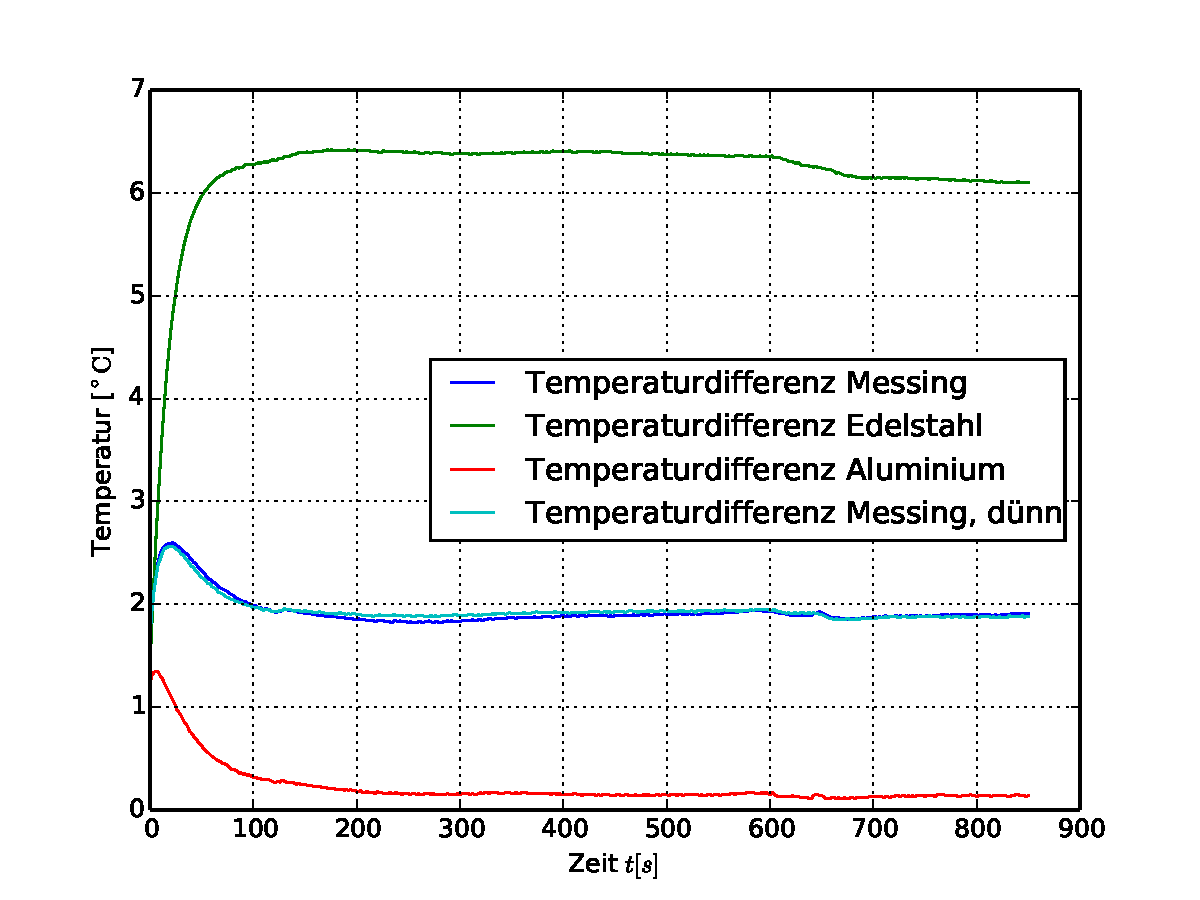
\includegraphics[width=0.8\textwidth]{Bilder/M1_Tempdiff.pdf}
	\caption{Temperaturdifferenz der Messpunkte von Messing und Edelstahl}
\end{figure}
Im Diagramm \ref{fig:tempverl} ist die Temperaturdifferenz innerhalb eines Stabes für den Edelstahl- und für den Messingstab aufgetragen. 
Es wird deutlich, dass die Differenzkurve für Edelstahl näherungsweise ein beschränktes Wachstum beschreibt und kurz nach Beginn der Erwärmung einen Grenzwert erreicht, der bei etwa  $6.25 \si{\degreeCelsius}$ liegt.
Die Differenzkurve des Messingstabes steigt zu Beginn der Messung an und erreicht kurz nach Beginn mit $2.6 \si{\degreeCelsius}$ ihr globales Maximum. 
Nach dem Maximum nimmt die Differenz exponentiell ab und erreicht einen Grenzwert von etwa $2 \si{\degreeCelsius}$.
Der Vergleich der Kurven zeigt, dass der Messingstab gegenüber dem Edelstahlstab den Grenzwert der Temperaturdifferenz schneller erreicht.

\subsection{Dynamische Messung mit 80 Sekunden-Periode}
Trolololo.